\documentclass{article}
\usepackage[utf8]{inputenc}
\usepackage{graphicx,tabularx}
\usepackage[a4paper]{geometry}
\usepackage{url}
\usepackage{listings}
\usepackage{amsmath}
\usepackage{mathtools}
\usepackage{algorithm}
\usepackage{algorithmic}
\lstset{language=Python}

\renewcommand{\algorithmicforall}{\textbf{for each}}

\title{The search for strong 4-cliques in Hollywood.}
\author{Thomas Snaidero (tsna), Jesper Jensen (jejen), Jonas Hinge (jhin)}
\date{December 2013}

\begin{document}

\maketitle

\section{Introduction}
The Academy awards is covered by thousands of journalist from all over the world, all of them competing for the best interviews. But what actors are the best fit for an interview and what actors could provide the best trivia?
To get the best interview with a possible best trivia, the journalist at the award show needs to know which actors are connected and how close or tight they are connected. This connection between actors in Hollywood has some resemblance to a social network.

\subsection{Hollywood as a social network}
A social network has multiple communities that ties the members of a social network together. The ties are based on one or more denominator eg. friends, collegues, home city or common interests.
The growth rate of a social networks density is commonly fast as every new node often is connected to a node already in the network and often bring adjacent nodes in to the network. In this assignment the Hollywood sceene is considered a social network of actors tied together by the movies they have appeared in together.

\subsection{Finding strong 4-cliques}
A 4-clique consist of 4 actors where each actor-pair has played in the same movie as shown in figure \ref{fig: 4clique example}.

\begin{figure}[H]
\begin{center}
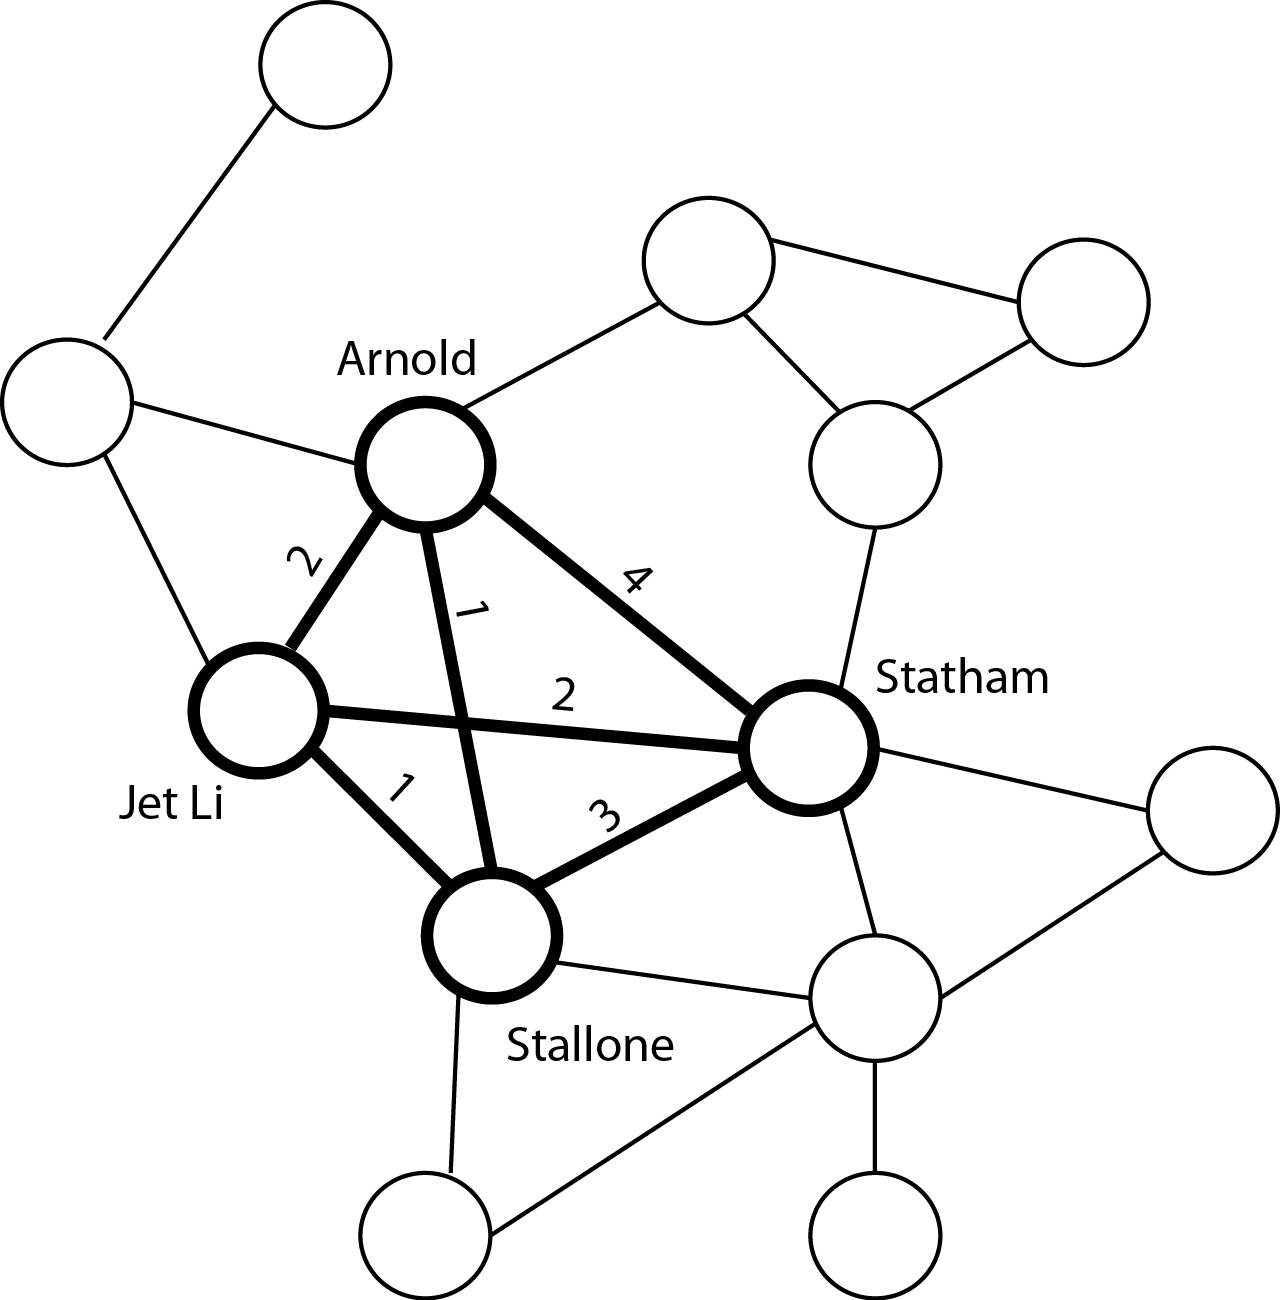
\includegraphics[scale=0.45]{graph_4clique.png}
\end{center}
\caption{\small {\it {4 clique example}}} 
\label{fig: 4clique example}
\end{figure}

We want to provide a tool, for finding the cliques of 4 actors that have strong ties to one another. The theses is: Stronger ties provides better gossip and stories from their clique. In order to find these cliques, we traverse the "social network" of Hollywood. This network is based on a cleaned IMDB dataset \cite{imdb}.
Each node in the graph is an actor. An Edge is formed if two actors have stared in the same movie. To define how strong the tie between these 2 actors is, we use the number of movies that they have stared together as weight on the edge between them. For a 4-clique, the strength of the clique is defined as the median value of the edges in the clique.

\subsection{Basic notations}
We define the hollywood social network as an undirected simple graph G with vertices or nodes V and edges E. The number of vertices $|V| = n$ and $|E| = m$. An edge is often in this project written as $\langle v,u\rangle$, a triangle as $\langle v,u,w\rangle$ and a 4-clique as $\langle v,u,w,z\rangle$. The vertices in these so called cliques are all interconnected i.e. each pair is connected.

We define a weight function $W(\langle v,u,w,z\rangle )$ for calculating how strong a 4-clique is. It simply returns the median of the edge weights (6 edge weights in a 4-clique).

We sometimes write $v_{adj}$ and this means the adjacent vertices of $v$.

\section{A sequential algorithm}
Developing a fast algorithm for finding strong 4-cliques has been an iterative process and we present 3 algorithms resulting from this; $strong\_4clique\_finder$ on page: \pageref{strong_clique}, $strong\_4clique\_finder+$ on page: \pageref{strong_clique_p} and $strong\_4clique\_finder++$ on page: \pageref{strong_clique_pp}. In all algorithms we keep track of the strongest clique throughout the computation and return it afterwards. There could exist 4-cliques with same weight - in this project we just return one of the strongest 4-cliques.

\subsection{Naive first attempt}
An intuitive first approach is the brute-force way. This algorithm simply checks for each vertex v in the graph if 3 adjacent nodes of v are interconnected i.e. there is a path between every node. The algorithm needs a graph G as input.

\begin{algorithm}
\label{strong_clique}
\caption{$strong\_4clique\_finder$}
\begin{algorithmic}
\REQUIRE $G$
\STATE $best\_clique = \langle empty\rangle $
\FOR{$v \in V$}
	\FOR{$u \in v_{adj}$}
		\FOR{$w \in v_{adj}$}
			\IF{$w \in u_{adj}$}
				\FOR{$z \in v_{adj}$}
					\IF{$z \in w_{adj}$ \AND $z \in u_{adj}$}
						\IF{$W(v,u,w,z) > W(best\_clique)$}
							\STATE $best\_clique = \langle v,u,w,z\rangle $
						\ENDIF
					\ENDIF
				\ENDFOR
			\ENDIF
		\ENDFOR
	\ENDFOR
\ENDFOR
\RETURN $best\_clique$
\end{algorithmic}
\end{algorithm}

\subsubsection{Analysis}
In the worst case a vertex v will have $n-1$ adjacent vertices, so for every v we have $O(n^{3})$ resulting in a total running time of $O(n^{4})$. This is not an attractive result as this easily could end up never executing especially with massive graphs with large n and m. We also note that as we are checking every node in a clique for all possible combinations to define this clique we actually count the same clique $4! = 24$ times.

\subsection{A better approach extending triangle counting}
Looking at NodeIterator++ \cite{countingTriangles} we see an effective and fast algorithm for finding triangles in a graph. A triangle is close to a 4-clique, we only need 1 node that in turn should be connected to all 3 nodes in the triangle.

\subsubsection{Intersection idea}
We see that if each node in a triangle has a common neighbour node this must close a 4-clique. So by intersecting the adjacent vertices of each vertex in a triangle and run through this intersection list, we can check for strong 4-cliques. Besides taking a graph as input this algorithm also needs a list of triangles $T$. These are found by NodeIterator++ \cite{countingTriangles}.

\begin{algorithm}
\label{strong_clique_p}
\caption{$strong\_4clique\_finder+$}
\begin{algorithmic}
\REQUIRE $G,T$
\STATE $best\_clique = \langle empty\rangle $
\FOR{$<v,u,w> \in T$}
	\STATE $intersection\_list = intersect(v_{adj}, u_{adj}, w_{adj})$
	\IF{$intersection\_list > 0$}
		\FOR{$z \in intersection\_list$}
			\IF{$W(v,u,w,z) > W(best\_clique)$}
				\STATE $best\_clique = \langle v,u,w,z\rangle $
			\ENDIF
		\ENDFOR
	\ENDIF
\ENDFOR
\RETURN $best\_clique$
\end{algorithmic}
\end{algorithm}

\subsubsection{Analysis}
We know from \cite{countingTriangles} that counting the triangles runs in $O(m^{3/2})$. For each triangle we make an intersection $O(n)$ and run through this intersected list $O(n)$ resulting in $O(2n)$ or just $O(n)$. So the total running time for finding strong 4-cliques is $O(nm^{3/2})$. We note that NodeIterator++ claims to count each triangle only 1 time. As a 4-clique contains 4 unique triangles and we are iterating all triangles, we see that each 4-clique is counted 4 times.

\subsection{Adapting the triangle counting approach}
We seek to optimize the algorithm further as we wish to count each 4-clique only 1 time. If we dig deeper into the triangle counting algorithm NodeIterator++ \cite{countingTriangles} we notice a method that could apply for finding 4-cliques as well.

\subsubsection{Lowest degree node responsibility}
Schank \cite{AlgorithmicAspects} proposed that the lowest degree node in each triangle be “responsible” for making sure the triangle gets counted. From this we define a lower degree function.

\begin{algorithm}
\label{strong_clique_p_wd}
\caption{$lower\_degree$}
\begin{algorithmic}
\REQUIRE $v,u$
\IF{$length(v_{adj)} < length(u_{adj})$}
	\RETURN $True$
\ELSIF{$length(v_{adj)} == length(u_{adj})$ \AND $id_{v} < id_{u}$}
	\RETURN $True$
\ELSE
	\RETURN $False$
\ENDIF
\end{algorithmic}
\end{algorithm}

We implement this degree function to the naive first algorithm so before iterating adjacent nodes we make sure that the lowest degree node is responsible for counting the possible 4-clique.

\begin{algorithm}
\label{strong_clique_pp}
\caption{$strong\_4clique\_finder++$}
\begin{algorithmic}
\REQUIRE $G$
\STATE $best\_clique = \langle empty\rangle $
\FOR{$v \in V$}
	\FOR{$u \in v_{adj}$}
		\IF{$lower\_degree(v,u)$}
			\FOR{$w \in v_{adj}$}
				\IF{$w \in u_{adj}$ \AND $lower\_degree(u,w)$}
					\FOR{$z \in v_{adj}$}
						\IF{$z \in w_{adj}$ \AND $z \in u_{adj}$ \AND $lower\_degree(w,z)$}
							\IF{$W(G,v,u,w,z) > W(best\_clique)$}
								\STATE $best\_clique = \langle v,u,w,z\rangle $
							\ENDIF
						\ENDIF
					\ENDFOR
				\ENDIF
			\ENDFOR
		\ENDIF
	\ENDFOR
\ENDFOR
\RETURN $best\_clique$
\end{algorithmic}
\end{algorithm}

\subsubsection{Analysis}
It can be proved that when using the lowest degree responsibility trick a vertex will have a degree of $O(\sqrt[]{m})$ \cite{AlgorithmicAspects}. As we are using this trick but in 4 nested iterations through the adjacent nodes of a vertex v we will end up with a running time of $O(\sqrt[]{m}\sqrt[]{m}\sqrt[]{m}\sqrt[]{m})$ or just $O(m^{2})$. We also note that this way ensures that each 4-clique is counted only 1 time as we in each iteration make 1 node responsible for completing the 4-clique.

\subsection{Space complexity}
For all 3 sequential algorithms we require a graph G as input. The running time complexity of the algorithms all assume that the graph G is build as an adjacency list so that for each vertice we have adjacent edges. This demands a space complexity of $O(mn)$. So running these sequential algorithms will require a very powerful machine with loads of memory as graph and especially social network graphs can be massive.


\subsection{Implementation and results}
We have implemented and compaired the sequential algorithms. The programming language used is Python 2.7 and the code is available at github \cite{gitcode}.

\subsubsection{Dataset and datastructure}
For building the graph we use an adjacency list consisting of a dictionary with vertices as keys and dictionaries as values. The value dictionaries have the adjacent vertices of the particular vertex as keys and their edge weight as values. The keys of the dictionaries are constructed with an actors id, firstname and lastname e.g. $actorid\_firstname\_lastname$.

\begin{lstlisting}

G = {426628_Arnold_Schwarzenegger : {
 		 {451117_Sylvester_Stallone : 6 },
 		 {452242_Jason_Statham : 2 },
 		 {277570_Jet_Li : 2 },
 		 { ... : ... }
 		}
 	},	
	{287328_Dolph_Lundgren : {
		 {451117_Sylvester_Stallone : 1 },
		 {487218_Jean-Claude_Van Damme : 4},
	 	 {277570_Jet_Li : 2 },
	 	 { ... : ... }
	 	}
	}
 \end{lstlisting}

\subsubsection{Results}

The implemented algorithms are benchmarked to measure the running time for each version of the algorithm, hence giving us the abillity to quantify the performance enhancement through each iteration. The first benchmark is performed on a small dataset - the dataset is then extended and benchmarked again.\newline

\textbf{IMDB Dataset : Year 2006 - 2008}
\begin{center}
    \begin{tabular}{ | l | l | l | l | l |}
    \hline
    Algorithm & N & M & Cliques & Runtime \\ \hline
    $strong\_4clique\_finder$ & 215 & 1040 & 60764 & 19.4 sec. \\ \hline
    $strong\_4clique\_finder+$ & 215 & 1040 & 60764 & 3 sec. \\ \hline
    $strong\_4clique\_finder++$ & 215 & 1040 & 60764 & 1.4 sec. \\ \hline
    \end{tabular}
\end{center}

\textbf{IMDB Dataset : Year 2005 - 2008}
\begin{center}
    \begin{tabular}{ | l | l | l | l | l |}
    \hline
    Algorithm & N & M & Cliques & Runtime \\ \hline
    $strong\_4clique\_finder$ & 8976 & 103939 & 12856587 & 4914 sec. \\ \hline
    $strong\_4clique\_finder+$ & 8976 & 103939 & 12856587 & 1123 sec.\\ \hline
    $strong\_4clique\_finder++$ & 8976 & 103939 & 12856587 & 713 sec. \\ \hline
    \end{tabular}
\end{center}

When we extend the dataset beyond 2005, the graph grows to large to process within resonable time on regular laptops.

\section{A parallel algorithm using MapReduce}

\subsection{MapReduce basics}
The algorithms that we have provieded are not able to process the entire graph due to memory exhaustion. To process the full dataset we will need an algorithmic approach that can run in parallel and traverse large datasets without hitting the upper memory barrier. MapReduce is a framework that wil provide the needed functionality and enable us to traverse the entire graph in a resonable running time.

\subsubsection{Map function}
The input in the map function is processed 1 tuple at a time. This allows distributing different tuples over multiple machines and creates the opportunity for massive parallelization. Each mapper emits a key,value pair which is then passed on to the shuffle phase.

\subsubsection{Shuffle}
The shuffle phase collects all key,value pairs and aggregates the pairs that have same key together. Finally it sends them on to the reduce phase on the same physical machine.

\subsubsection{Fold (Reduce) Function}
The reducer processes each key along with all of its values associated with it together. In this step operations on data with a specific key are independent of data with other different keys which means that like in the map phase this step can be parallelized.

\subsection{Finding strong 4-cliques using MapReduce}
We come with a suggestion for finding strong 4-cliques with MapReduce. It is strongly inspired from the improved MapReduce triangle counting algorithm from lecture slides on MapReduce \cite{lnMapReduce} and from MR-NodeIterator++ \cite{countingTriangles}. We basically extend the algorithm so instead of counting the triangles we search for strong 4-cliques but using the same techinques as for triangle counting.

\subsubsection{Suggestion for an algorithm}
The idea of the algorithm is basically the same as for the sequntial $strong\_4clique\_finder++$ algorithm but now, in order to distribute data from the graph to different machines, we split up the computations into 3 map/reduce iterations or rounds. For emitting and receiving the data we use key/value pairs e.g. $\langle vertex1,vertex2\rangle :\$$ where the key is an edge pair. The $\$$ sign defines a possible value.

\paragraph{Round 1}
In the first round we map edges from the graph, but using the lowest degree function we ensure that we only emit the same edge once e.g. $\langle v,u\rangle$ and not $\langle u,v\rangle$ assuming that in this case $v$ has a lower degree than $u$. We also emit a key/value pair $\langle v,\$\rangle :u$ where the key is a possible edge pair and $u$ is an adjacent node. In this way we make $v$, the lowest degree node, responsible for finding a node that closes the triangle and later on the 4-clique. After some shuffling the reducer will receive a list of adjacent nodes for one possible edge $\langle v,\$\rangle$ and from this list we emit paths e.g. $\langle x,y\rangle :v$ and again make sure that we don't emit the same edge twice using $lower\_degree(x,y)$. By doing this we also ensure that the ordering of $v,u$ is the same as the emitted $emit(\langle v,u\rangle :\$)$ as these keys needs to match in order to collect adjacent values in a list in the following rounds. If the value is $\$$ we just propogate the key/value pair to the next round.

\paragraph{Round 2}
We simply propogate the pairs in the mapping phase of round 2. In the reducer we check that the pairs emitted from round 1 is actually connected. This is done by removing and propogating the $\$$ from the pair $\langle v,u\rangle$ and if there are still values left, these are the vertices that connects to both vertices in the pair i.e. they close a triangle. We then iterate as in round 1 through these adjacent nodes and emit possible pairs, only this time with the key pair as value e.g. $\langle x,y \rangle :\langle v,u \rangle$.

\paragraph{Round 3}
As for the last round we simply propogate pairs in the mapper of round 3. In the reducing part we need to check, like in the triangle case last round, if the possible pairs we emitted are actually connected. If they are they will close a 4-clique. We do this by checking if there exist a $\$$ in the value list of the possible pairs and if so, we remove it and iterate through the list. This time the values will be pairs $\langle w,z \rangle$ and they are the ones closing a 4-clique $\langle v,u,w,z \rangle$. While iterating we keep track of the 4-clique with max weight. The pseudo code of the algorithm $mr\_strong\_4clique\_finder$ is shown on page \pageref{mrAlgorithm}.

\begin{algorithm}
\label{mrAlgorithm}
\caption{$mr\_strong\_4clique\_finder$}
\begin{algorithmic}
\REQUIRE $G$
	
\REQUIRE MAP 1: $\langle v,u\rangle :\$$
	\IF{$lower\_degree(v,u)$}
		\STATE $emit(\langle v,\$\rangle :u)$
		\STATE $emit(\langle v,u\rangle :\$)$
	\ENDIF
\REQUIRE REDUCE 1: $\langle v,u\rangle :u_{adj} = [u_1,u_2,...]$
	\IF{$u != \$$}
		\STATE $emit(\langle v,u\rangle :\$)$
	\ENDIF
	\FOR{$x \in u_{adj}$}
		\FOR{$y \in u_{adj}$}
			\IF{$lower\_degree(x,y)$}
				\STATE $emit(\langle x,y\rangle :v)$
			\ENDIF
		\ENDFOR
	\ENDFOR

\REQUIRE MAP 2: $\langle v,u\rangle :w$
	\STATE $emit(\langle v,u\rangle :w)$
\REQUIRE REDUCE 2: $\langle v,u\rangle : vu_{adj} = [vu_1,vu_2,...]$
	\IF{$\$ \in vu_{adj}$}
		\STATE $emit(\langle v,u\rangle : \$)$
		\STATE remove \$ from $vu_{adj}$
	\ENDIF
	\FOR{$x \in vu_{adj}$}
		\FOR{$y \in vu_{adj}$}
			\IF{$lower\_degree(x,y)$}
				\STATE $emit(\langle x,y\rangle :\langle v,u\rangle)$
			\ENDIF
		\ENDFOR
	\ENDFOR

\REQUIRE MAP 3: $\langle v,u\rangle :wz$
	\STATE $emit(\langle v,u\rangle :wz)$
\REQUIRE REDUCE 3: $\langle v,u\rangle :wz = [wz_1,wz_2,...]$
	\STATE $best\_clique = \langle empty\rangle $
	\IF{$\$ \in wz$}
	\STATE remove \$ from $wz$
		\FOR{$\langle w,z\rangle \in wz$}
			\IF{$W(\langle v,u,w,z\rangle) > W(best\_clique)$}
				\STATE $best\_clique = \langle v,u,w,z\rangle$
			\ENDIF
		\ENDFOR
	\ENDIF
\end{algorithmic}
\end{algorithm}

\subsubsection{Analysis}
We use 4 parameters when analysing the mapreduce algorithm; round numbers, total work, work per reducer and pair numbers. We notice that by using the lower degree responsibility we reduce the size of possible adjacent vertices for a node to $O(\sqrt[]{m})$ according to the same proof \cite{AlgorithmicAspects} used in the sequential algorithm $strong\_4clique\_finder++$. With this way we also make sure that each 4-clique is only counted 1 time.

\paragraph{Round numbers}
As a mapreduce round can involve shuffling terabytes of data the number of rounds should remain constant or in the worst case logarithmic. In our case we stay at 3 rounds constantly.

\paragraph{Work per reducer}
The reducer with the worst running time. In our case we have round 1 and round 2 as the worst rounds. They both double iterate through possible adjacent nodes so the running time is $O(\sqrt[]{m}\sqrt[]{m})$ or just $O(m)$.

\paragraph{Total work}
The total work is the worst running time for a round. Round 1 and round 2 are both $O(m)$ and the number of pairs to examine is the max number of edges $O(\sqrt[]{m})$ so in total $O(m\sqrt[]{m})$.

\paragraph{Pair numbers}
Pair numbers describe the max number of pairs we map in a round. This is important to keep as low as possible as the shuffling operation can be very expensive. The max number of pairs are emitted from the reducer in round 1 and 2 and propogated by the next round mapper so the shuffling between round 1 and 2 and round 2 and 3 will receive pair numbers of $O(m\sqrt[]{m})$. The bound is calculated from the fact that the reducer receives $O(m)$ key,value pairs and each of these can have $O(\sqrt[]{m})$ adjacent nodes (or edge pairs in round 3).

\section{Conclusion}
We have in this project explored different ways of constructing algorithms that returns the strongest 4-cliques in a graph. After 3 iterations we developed a sequential algorithm that is optimal in the sense that it only counts the 4-cliques 1 time each. We discovered a running time of $O(m^{2})$ running this algorithm. For this we use $O(mn)$ space and by implementing and testing this we quickly discovered that bigger machines are required and must importantly multiple machines i.e. we need to parallelize the algorithm.
We then gave a suggestion for a parallel algorithm using MapReduce. Assuming the algorithm will work in practice we analyzed the algorithm and found complexities of the following parameters; round numbers: 3, work per reducer: $O(m)$, total work: $O(m\sqrt[]{m})$ and pair numbers: $O(m\sqrt[]{m})$.
For future improvements one could consider using the edge weights to construct a heuristic that can prune some of the edges and decrease the amount of data.


\begin{thebibliography}{1}

\bibitem{imdb}
    Rasmus Pagh and Francesco Silvestri
    \emph{Description of the IMDb and MovieLens datasets}
    \url{https://blog.itu.dk/SAD2-E2013/files/2013/10/datasets.pdf}

\bibitem{lnMapReduce}
    Lecture notes: MapReduce
    \emph{MapReduce}
    \url{https://blog.itu.dk/SAD2-E2013/files/2013/11/mapreduce.pdf}

\bibitem{countingTriangles}
    Siddharth Suri and Sergei Vassilvitskii
    \emph{Counting Triangles and the Curse of the Last Reducer}
    \url{http://theory.stanford.edu/~sergei/papers/www11-triangles.pdf}

\bibitem{AlgorithmicAspects}
    Thomas Schank
    \emph{Algorithmic Aspects of Triangle-Based Network Analysis}
    \url{http://digbib.ubka.uni-karlsruhe.de/volltexte/documents/4541}

\bibitem{gitcode}
    Thomas Snaidero, Jesper Jensen and Jonas Hinge
    \emph{Python code for sequential algorithms for finding 4-cliques}
    \url{https://github.com/jplay83/SAD2/blob/master/jonas/max_weighted_4clique.py}
    
\end{thebibliography}

\end{document}



% TODO INTERNAL
% figure description on algorithms
% references
% implementation
% run algorithm and note down running times
% conclusion
% READ and CORRECT
% print
% READ and CORRECT
% print



